\documentclass[11pt]{article}
\usepackage[left=1in, right=1in, top=0.75in, bottom=1in]{geometry}
\usepackage{mathexam}
\usepackage{amsmath}
\usepackage{graphicx}
\usepackage[export]{adjustbox} %positioning of images
\usepackage[dvipsnames]{xcolor}
\usepackage{enumitem}
\usepackage{setspace}
\usepackage{latexsym}
\usepackage{wasysym}
\usepackage{amssymb}
\usepackage{pgfplots}
\usepackage{comment}
\usepackage{exsheets}
\usepackage{pdfpages}
\usepackage{multicol}

\ExamClass{Math 242}
\ExamName{Classwork 08: \S 11.1-11.2}
\ExamHead{Fall 2024}
\fancyfoot{}
\setlength{\headheight}{13.59999pt}

\let\ds\displaystyle
\newcommand{\ddx}{\frac{d}{dx}}
\newcommand{\red}{\textcolor{red}}
\newcommand{\blue}{\textcolor{blue}}
\newcommand{\pink}{\textcolor{CarnationPink}}
\newcommand{\orange}{\textcolor{orange}}
\newcommand{\purple}{\textcolor{purple}}
\newcommand{\violet}{\textcolor{violet}}
\newcommand{\cyan}{\textcolor{cyan}}
\newcommand{\grn}{\textcolor{green}}
\newcommand{\uh}{\textcolor{ForestGreen}}
\newcommand{\bas}[1]{\begin{align*}{#1}\end{align*}}

\pgfplotsset{compat=1.18}

\pgfplotsset%Default tikz axis style
{
    axis lines=center, 
    grid,
    grid style={very thin, densely dotted, black!50},
    xmin=-5,    xmax=5,         xtick distance=1,
    ymin=-5,    ymax=5,         ytick distance=1,
    restrict y to domain=-10:10, % <-------
    ticklabel style={font=\scriptsize, fill=white, inner sep=2pt},
    domain=-5:5, samples=100,
    no marks, 
    every axis plot post/.append style={ultra thick, semitransparent,},
}

\pgfkeys{/pgfplots/Axis Style/.style=
{
    grid style={thin, densely dotted, black!50},
    width=11.5cm, height=5cm,
    axis x line=center, 
    axis y line=middle, 
    samples=100,
    ymin=-1.1, ymax=1.1,
    xmin=-.1, xmax=6.4,
    domain=0:2*pi
}}

\def\myalign#1{%
  \def\trule{\noalign{\smallskip\hrule\medskip}}
  \def\nebc{\nearrow\bigcup}
  \def\sebc{\searrow\bigcup}
  \def\pminf{{}_{-\infty}|^{+\infty}}
  \let\Inf\infty
  \def\amp{&}% props to Bruno; I just love this trick
  \vbox{\mathsurround0pt\openup1\jot
    \halign{%
      &$\displaystyle##\hfil\tabskip0pt$&\amp##\tabskip1em\crcr
      \noalign{\hrule height1pt\smallskip}#1\noalign{\smallskip\hrule height1pt}\crcr}}}

\linespread{1.3}

\begin{document}

    \hrule
    \vspace{.5cm}
    \noindent\textbf{Name:} \underline{\qquad\qquad\qquad\qquad\qquad\qquad\qquad\qquad\qquad\qquad\qquad\qquad\qquad}

    \begin{enumerate}
        \item Do the following \textbf{sequences} $\{a_{n}\}$ converge or diverge? If they converge, what do they converge to? Justify your answers.
        \begin{enumerate}
            \item $a_{n}=\ds\frac{e^{n}}{3^{n}}$\vfill
            \item $a_{n}=(-1)^{n}\sqrt{n}$\vfill
            \item $a_{n}=\ds\frac{(-1)^{n}+n}{(-1)^{n}-n}$\vfill
            \item $a_{n}=(-1)^{n}\sin\left(\frac{\pi}{2}(2n+1)\right)$\vfill
        \end{enumerate}
        \newpage
        \item Consider the figure:
        \begin{center}
            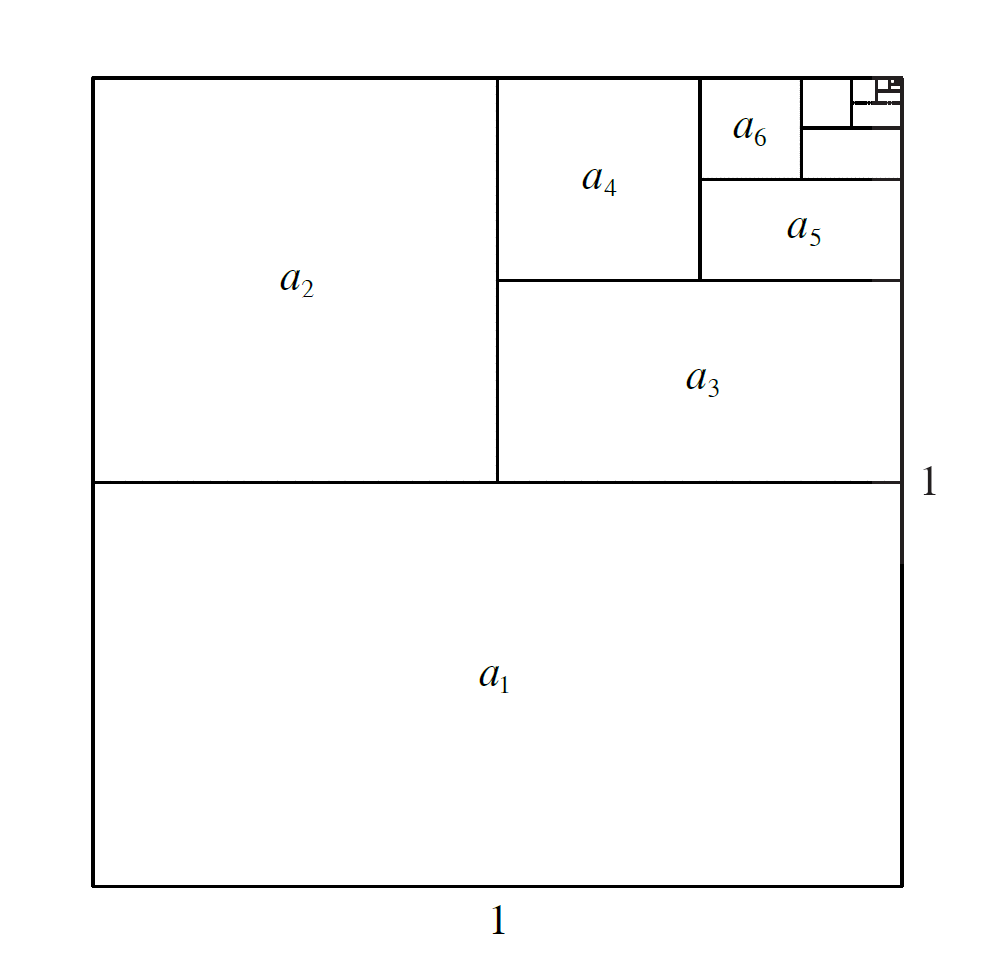
\includegraphics[width=10cm]{F24/Classwork 08/ws08.1.png}
        \end{center}
        \begin{enumerate}
            \item Find a general expression for the area of the $n$th shape, $a_{n}$.\vfill
            \item What is $\ds\sum_{n=1}^{\infty}a_{n}$.\vfill
        \end{enumerate}
        \newpage
        \item Consider the series $\ds\sum_{i=1}^{\infty}\ds\frac{1}{i}$.
        \begin{enumerate}
            \item What are the first ten partial sums $s_{n}$? (use of a calculator is alright for this problem)
            \begin{center}
                \begin{multicols}{2}
                    $s_{1}=\underline{\phantom{...............}}$\\[1em]
                    $s_{2}=\underline{\phantom{...............}}$\\[1em]
                    $s_{3}=\underline{\phantom{...............}}$\\[1em]
                    $s_{4}=\underline{\phantom{...............}}$\\[1em]
                    $s_{5}=\underline{\phantom{...............}}$\\[1em]
                    
                    $s_{6}=\underline{\phantom{...............}}$\\[1em]
                    $s_{7}=\underline{\phantom{...............}}$\\[1em]
                    $s_{8}=\underline{\phantom{...............}}$\\[1em]
                    $s_{9}=\underline{\phantom{...............}}$\\[1em]
                    $s_{10}=\underline{\phantom{...............}}$\\[1em]
                \end{multicols}
            \end{center}
            
            \item On the graph below, plot $(n, s_{n})$ for the above values.
            
            \begin{center}
                \begin{tikzpicture}
                    \begin{axis}[scale=2, xmin=-.5, xmax=10.5, ymin=-.5, ymax=4.5, ytick distance=.25, xtick distance =.5] 
                        
                    \end{axis}
                \end{tikzpicture}
            \end{center}
            \item On the same axes, graph $y=\ln(x)$ and $y=\ln(x)+1$. (yes, you can use a calculator for this as well)
            \item Looking at the graph of the sequence of partial sums, will this series converge or diverge? If it converges, what does it converge to?
        \end{enumerate}
    \end{enumerate}

\end{document}